\subsection{Probes}

A system instrumented with OpenTelemetry has spans and traces to observe the execution of an operation \cite{otel-t}. The same level of observability must be assured in the oscilloscope, this is why we provide the concept of probes, which, like spans, follow an execution from start to end. \textbf{Note} that a definition of probes has already been introduced in a previous article relating to $\Delta$QSD \cite{dq-br}, but the concept we present here is not the same.

To observe a system, we must put probes in it. For each outcome of interest, a probe (observation point) is attached to measure the delay of the outcome, like one would in a true oscilloscope \cite{post}.

Consider the figure below, a probe is attached at every component to measure their $\Delta$Qs ($p_2, p_3$),  Another probe ($p_1$) is inserted at the beginning and end of the system to measure the global execution delay. Thanks to this probe, the user can observe the $\Delta$Q \textit{``observed at $p_1$''}, which is the $\Delta$Q which was calculated from the data received by inserting probe $p_1$. The \textit{$\Delta$Q ``calculated at $p_1$''} is the resulting $\Delta$Q from the convolution of the observed $\Delta$Qs at $c_2$ and $c_3$. \\
Probe $p_1$ is the equivalent of a ``root/parent span'' which observe the whole execution of $c_1, c_2$, while $p_2$ and $p_3$ are child spans which represent single instances of execution.

    \begin{figure}[H]
        \begin{center}
            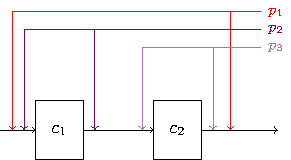
\includegraphics[scale=1.8]{tikz/probes.pdf}
        \end{center}
        \caption{Probes inserted in a component diagram. In an application instrumented with OpenTelemetry, $p_1$ could be considered the root span, $c_1$ and $c_2$ its children spans sharing a causal link.}
        \label{fig:probes}
    \end{figure}



